% Project report for the AstroML course - Spring 2016 - SU
\documentclass[a4paper, 11pt]{article}
\usepackage{graphics,graphicx}
\usepackage{natbib}
\bibliographystyle{unsrtnat}
\oddsidemargin=-0.54cm
\evensidemargin=-0.54cm
\topmargin=-1.2cm
\textwidth=17cm
\textheight=25cm
\pagestyle{empty}

\begin{document}

\begin{titlepage}
   \vspace*{\stretch{1.0}}
   \begin{center}
      \LARGE\textbf{A machine learning approach to time delay estimation -- case of gravitationally lensed quasars}\\
      \vspace{20mm}
      \Large\textsc{AstroML Course Project Report}\\
      \Large\textsc{Department of Astronomy, Stockholm Univeristy}\\
      \vspace{50mm}
      \Large\textbf{\textit{Saghar Asadi}\\}
      \vspace{20mm}
      \Large\textit{May 2016}
   \end{center}
   \vspace*{\stretch{2.0}}
\end{titlepage}

\section{Abstract}
Two years ago, a challenge was proposed (http://timedelaychallenge.org/), that simulated a large number of lensed quasar light curves in which the participants had to measure the time delay of the system blindly (no data about the lens system, or the host AGN, or microlensing events).  Several groups competed with different algorithm to derive time delays and at the end of the challenge, the organizers published the simulated light curves along with the ground truth of the systems (the true time delay, macrolens image magnitudes, the characteristic time delay, and the characteristic magnitude of fluctuations for each system). Our goal is to train a regression algorithm to derive time delays using the labelled light curves (TDC1). The expectation is that this will give better results than the blind estimation, and given a representative set of simulations as the training set, could be used on large data sets (such as those monitored by \citep{LSST+2009}), which in return provides a robust measurement for the accelerating expansion of the Universe (for the proposed method see \citet{Refsdal1964}).

This is a report on the partial progress of the project so far. This project is still in progress!

\section{Introduction to the data}

The simulated light curves are generated based on a plausible distribution of physical parameters of the main lens and there is a total number of 1024 published lens systems with the ground truth information as mentioned above; including 760 doubly--imaged lens systems and 152 quadratic systems. Since systems with more than two images need a different analysis, we have removed them from our training sample for the time being.

The true time delays are in a range between 5 to 120 days, and the analysis of competing algorithms show that true time delays below ~10 days allow for few accurate measurement. On the other hand, our results at this stage also seems to suggest that the length of the continuous sampling of the light curve also puts an upper limit on the time delay estimation.

\subsection{Raw data}
The process of generating the data used in this project can be found in details in \citet{Liao+2014} and summarized in figures 3 and 4 of the same paper. The process includes 4 main steps:
\begin{itemize}
  \item Generating the intrincis time variation of the AGN (the source), so that tha total sample is representative of the physical parameter space.
  \item Adding the microlensing events along the line of sight of each image. The total microlensing effect is a combination of an unknown number of independent microlensing events that effect each image of the source independently and therefore should only be treated statistically.
  \item Filtering the light curves with sampling windows (simulating the effect of observations). Therefore the continuous light curves are resampled in specific time stamps in unequal timesteps.
  \item Adding the observational noise as uncertainties in the flux measurements for each data point.
\end{itemize}

\subsection{Ground truth information}
The ground truth information about each simulated system including the true time delay in days (dt), the true magnitueds of each image of the quasar in magnitudes ($m_1$ and $m_2$), the lens and source redshifts ($z_l$, and $z_s$), and the typical intrinsic variation of the AGN in time ($\tau$) and flux ($\sigma$) are provided in separate datasets.

\begin{figure}
\centering
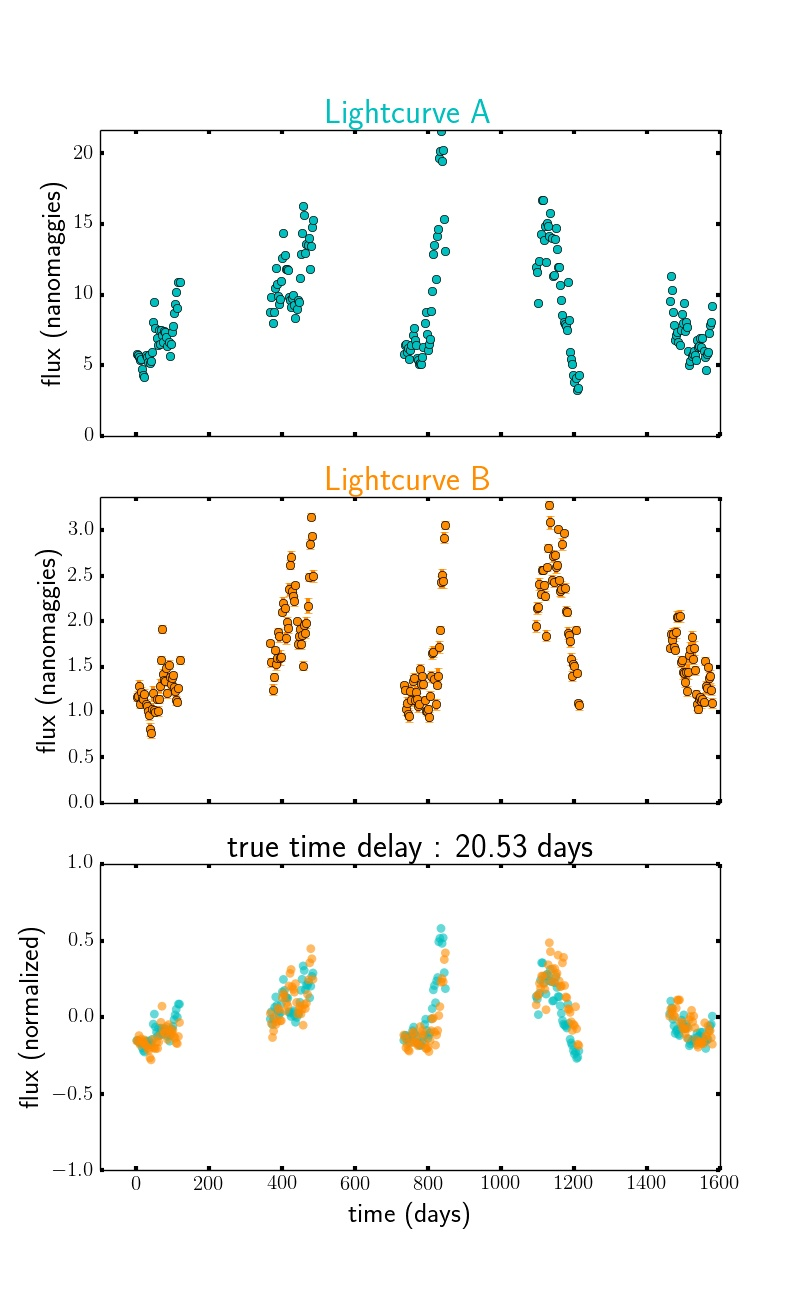
\includegraphics[width=0.49\textwidth]{Figures/Fig1.jpg}
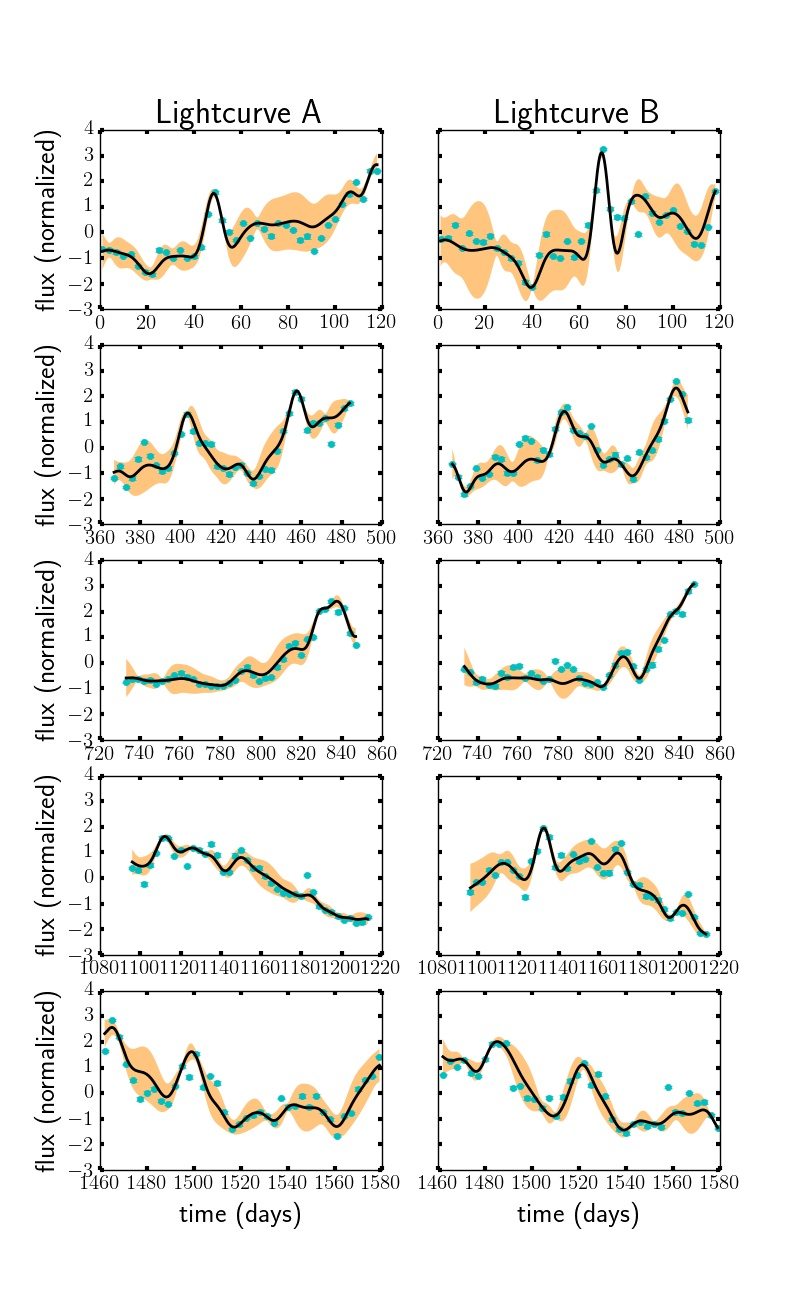
\includegraphics[width=0.49\textwidth]{Figures/Fig2.jpg}
\caption{{\bf (Left) }An example of our raw data. The two top panels plot the two light curves of the same pair with measured errorbars, while the bottom panel overplots the centerd and normalized light curves, as we work with throughout this project. {\bf (Right) }The same data set as the one shown in the left panel of figure \ref{fig:Fig1}. Each row in the above figure is a close-up of each of the sampling windows in the data set which is fed to a Gaussian Process regression (as explained in section XX). In each subplot, the cyan errorbars are measured data points, while the thick black curve is the best-fit smooth model of the signal, and the orange region indicates the 95\% uncertainty region of the model. Note that the data that go into the Gaussian Process Regressor is centered and normalized, and each light curve in each window is smoothed independently of the other.}
\label{fig:Fig1}
\end{figure}

\section{Method}
\subsection{Overall strategy}

The main purpose of this project is to find a way to improve the accuracy of the time delay estimators proposed within the main challenge using the ground truth information. Our proposed idea can be summarized in 5 basic steps (excluding the first step that is considered as pre-processing the data):

\begin{enumerate}
  \item Split light curves into continuous observation windows (pre--processing)
  \item Smooth the light curves and interpolate evenly sampled data
  \item Compare the two light curves of each window for each timesift
  \begin{itemize}
    \item Find the best timeshift for each window
  \end{itemize}
  \item Compare the estimated time delays of different windows of the same pair
  \item Use a clustering algorithm to cluster the results
  \item Apply a regression method to the clustered values
\end{enumerate}

\subsubsection{Smooth the light curves and interpolate evenly sampled data}
We smoothed each observing window for each light curve individually using a Gaussian Process, using tau and sig from the ground truth. It is however also possible to optimize the smoothing by cross validation. We not only solve the problem of the raw time series being unevently-sampled in time, but also keep error estimate in this step.

\subsubsection{Compare the two light curves of each window for a range of timeshifts}
The standard method to derive the time delay between two signals is to compare the two signals by keeping on constant, and shifting the other by a range of time steps. The cost function for this method could be defined in various forms, and the timeshift resulting in the minimum cost would result in the estimated time delay between the two signals.

We compared the two light curves of each window for each possible timeshift of one curve relative to the other using two different methods:
\begin{itemize}
  \item Correlation: First, we measure the cross correlation using the pre difined \emph{scipy.signal.correlate} function using \emph{mode='full'} and maximize the correlation coefficient for the timeshift.
  \item Mean squared error: 
Secondly, we measure the mean squared difference btween the signals at each time window for timeshifts between - window length and + window length. The estimated time delay according to this method is the timeshift resulting in the minimum value for the MSE.
\end{itemize}

\begin{figure}
\centering
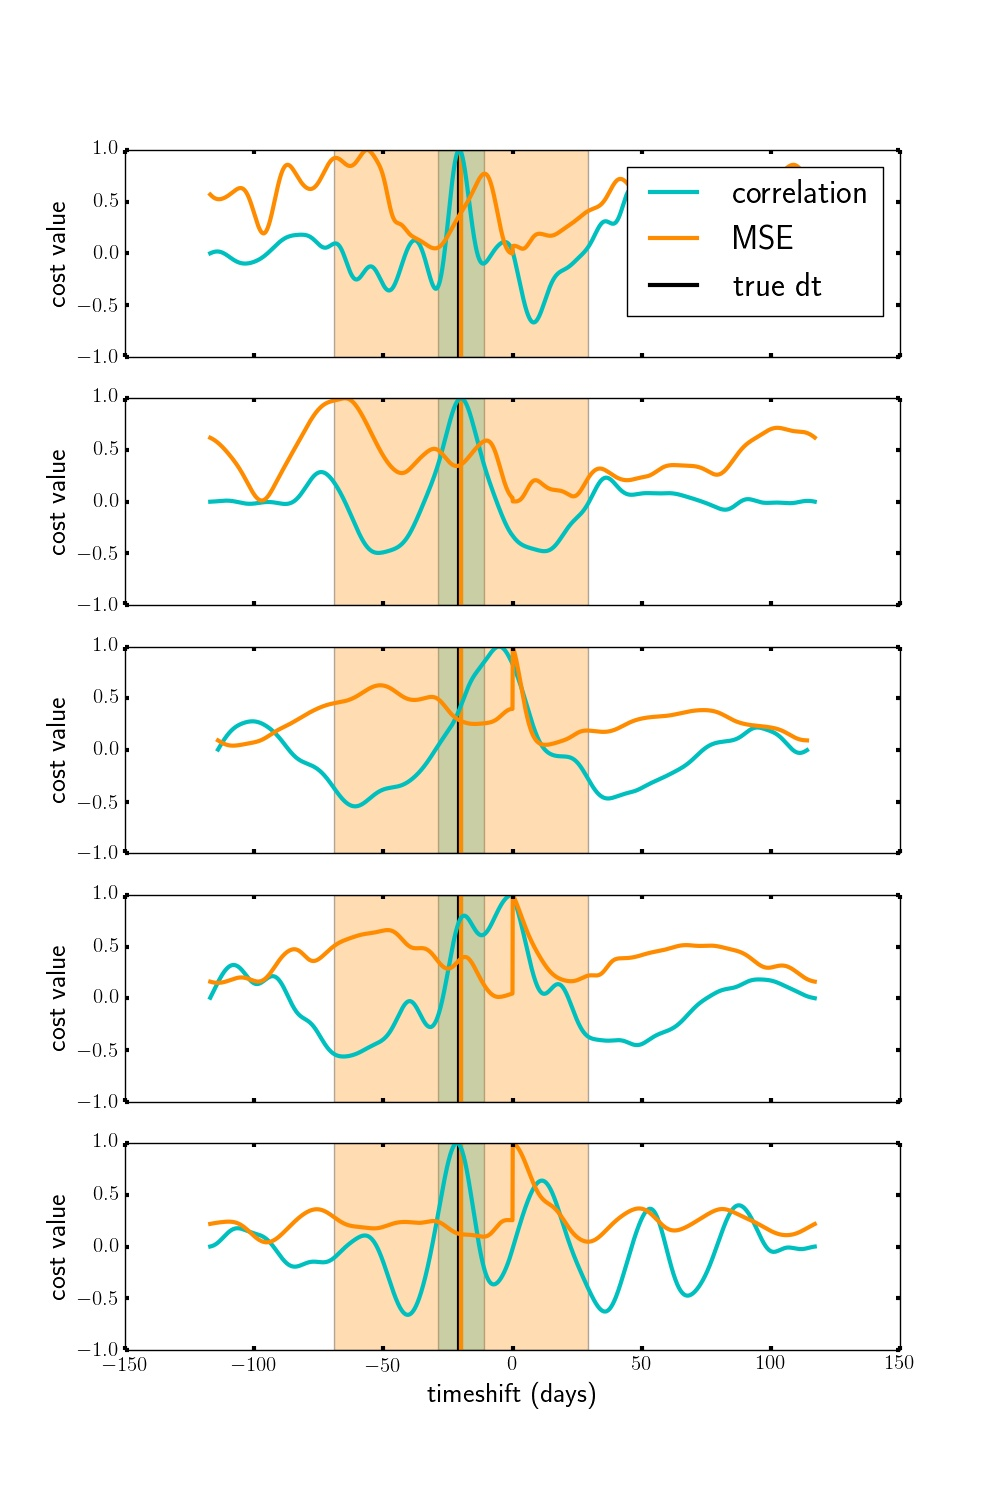
\includegraphics[width=0.49\textwidth]{Figures/Fig31.jpg}
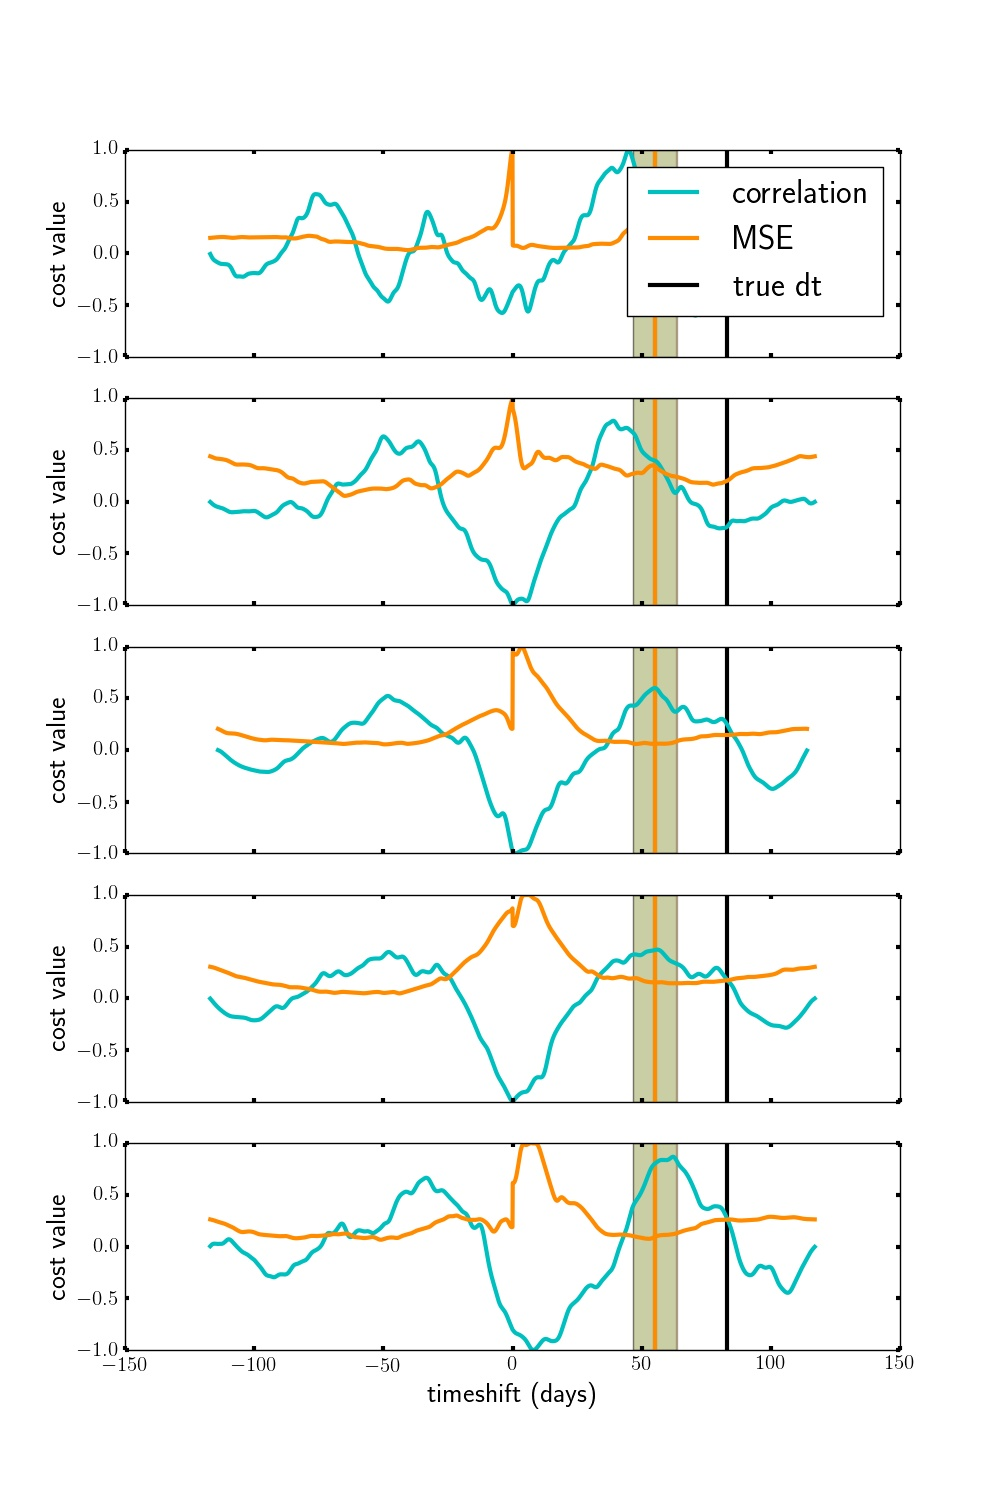
\includegraphics[width=0.49\textwidth]{Figures/Fig32.jpg}
\caption{{\bf (Left) }An example of correlation and MSE values for different timeshifts between the two signals. The orange curve indicate the measured mean-squared-error between the two signals at a given timeshift (x axis), and the cyan curve shows the correlation coefficient between the two signals at each timeshift. The vertical lines of each color are indicators of the median value of the time delays derived from each observing window, corresponding to the same method (i.e. orange for MSE and cyan for correlation). The black vertical line marks the true time delay of the system given by the ground truth information. In this system, both metods seem to be consistently predicting the time delay as $\sim -20$ days while the true value is 20.53 days. However, the values derived from MSE measurements are far less accurate. {\bf (Right) }An example of correlation and MSE values for different timeshifts between the two signals. The orange curve indicate the measured mean-squared-error between the two signals at a given timeshift (x axis), and the cyan curve shows the correlation coefficient between the two signals at each timeshift. The vertical lines of each color are indicators of the median value of the time delays derived from each observing window, corresponding to the same method (i.e. orange for MSE and cyan for correlation). The black vertical line marks the true time delay of the system given by the ground truth information. In this system, even though both measurements are consistent in the median and standard deviation of the measurements, the true time delay of the system does not lie within the uncertainty region of our estimated time delay.}
\label{fig:Fig3}
\end{figure}

\subsubsection{Compare the estimated time delays of different windows of the same pair}
The maximum correlation offsets for different windows can vary quite a lot for the same system. However, the standard deviation of the time delay estimations across windows for the same system seems to be correlated with the true time delay. The reason for this correlation could be explained with the two following edge cases:

\begin{itemize}
  \item if $dt_\mathrm{true} \geq$ sample window size: With $dt_\mathrm{true} \geq$ sample window size, there is no overlap at all between the two signals inside any window, and any correlation between the two signals at any offset is only random (i.e. due to the noise or microlensing effect). The variance of the timeshift at which the correlation is at maximum across windows is therefore high.
  \item if $dt_\mathrm{true} = 0$: The whole of the two signals match each other at an offset $ = dt_\mathrm{true} = 0$, and any other high correlation is only due to microlensing and noise. Thus the variance of the timeshift at which the correlation is at maximum across windows is is low, and would be 0 if there was no noise or microlensing effects.
\end{itemize}

Therefore, in between these two extreme cases, the variance of the timeshift at which the correlation is at maximum across windows should is correlated to $dt_\mathrm{true}$.

To capture this dynamic, we calculated both the mean and median as well as the standard deviation of the maximum correlation offsets within each pair, weighting the maximum correlation offset of each window by its correlation coefficient.

Additional problems with time delay estimation directly from the correlation coefficients:

\begin{itemize}
  \item Each light curve has experienced microlensing events that are independent of those of the other image
  \begin{itemize}
    \item solution: account for microlensing events in a statistical way rather than individually 
    \item the far-fetched proposed solution: train a classifier (maybe a neural network) on the microlensing events and subtract a range of typical microlensing events from both signals, and use cross validation to choose the best microlensing effect by maximizing the cross correlation coefficients.
  \end{itemize}
  \item We have no information about the effect of microlensing effects, they could only influence the trend of the data, so may be removed by detrending the light curves before cross correlating them, but the added peaks are impossible to be accounted for indicidually, but only in a statistical sense
  \begin{itemize}
    \item solution: work with centred, normalized, and detrended light curves
  \end{itemize}
\end{itemize}

\subsubsection{Use a clustering algorithm to cluster the results}
The results from the previous step contain a lot of noise, which needs to be removed in order to use them to train the final regressor. The noise in the estimated time delays can be significantly improved by using a clustering algorithm such as nearest neighbour on the correlation offset measures. The algorithm finds the $dt_i$ value maximizing the expression below, as the representative feature for any given $dt_\mathrm{true}$:

\begin{equation}
\Sigma_{j}\frac{1}{1 + (dt_i - dt_j)^2}
\end{equation}

\begin{figure}
\centering
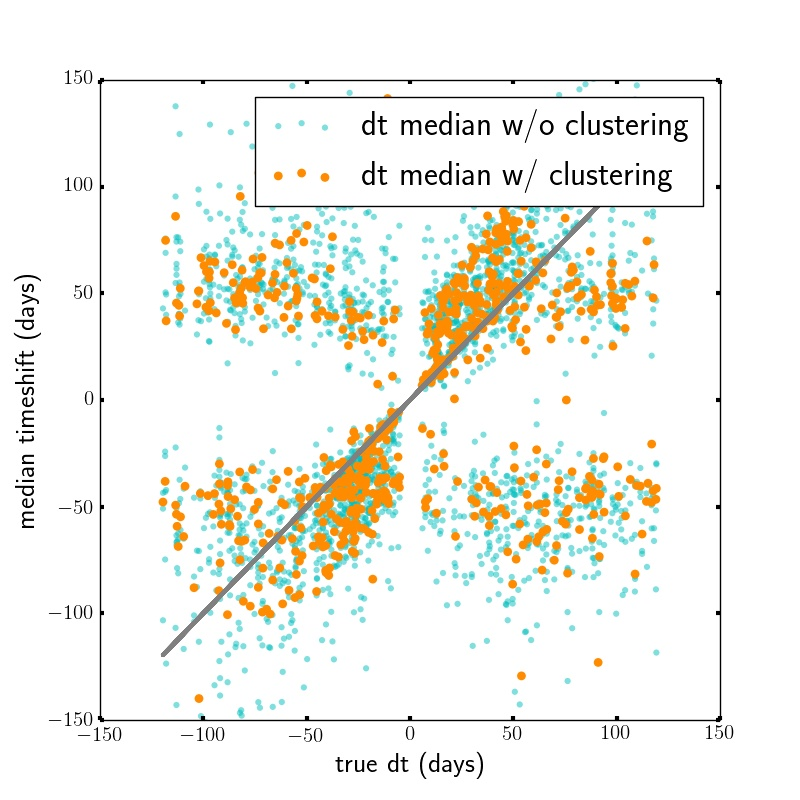
\includegraphics[width=0.49\textwidth]{Figures/Fig4.jpg}
%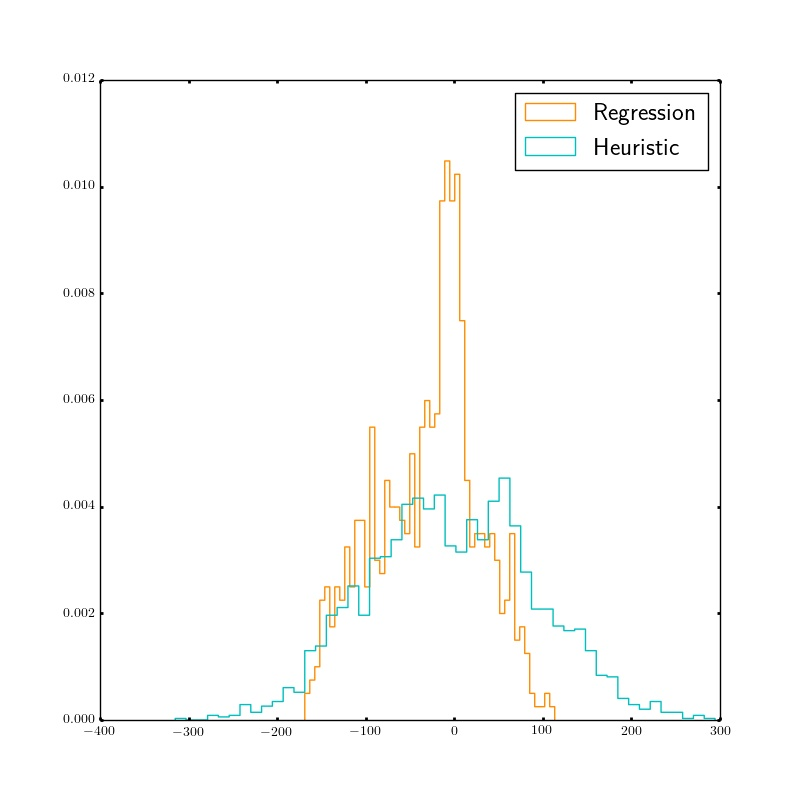
\includegraphics[width=0.49\textwidth]{Figures/Fig6.jpg}
\caption{A scatter plot showing the effect of clustering on the time delay estimated by correlation/MSE methods.}% {\bf (Right )} Priliminary results of linear regression trained on a clustered data set. The cyan histograms are the distribution of the mean squared difference between the estimated time delays and $dt_\mathrm{true}$s for a test set, while the orange histogram is the same difference between }
\label{fig:Fig4}
\end{figure}

\subsubsection{Apply a regression method to the clustered values}
We used a regression algorithm with the maximum correlation coefficients and MSE of the two light curves as features for the entire pair, using $dt_\mathrm{true}$, as well as other ground truth information we have
as the labels, hoping to do a multi-dimensional regression. Even though the clustered training set show much lower noise, linear regression fails to find a good fit to the training set. One reason is thought to be the large fraction of estimated time delays with the wrong sign. This is expected to be cases such as that shown in the right planel of figure \ref{fig:Fig3} where neither of the correlation nor MSE curves seem to show a significant assymetry in the local extrema.

This part is a work in progres...

\newpage
\begin{thebibliography}{}
\bibitem[Liao et al.(2015)]{Liao+2014} Liao, K., Treu, T., Marshall, P., et al.\ 2015, ApJ, 800, 11 
\bibitem[LSST Science Collaboration et al.(2009)]{LSST+2009} LSST Science Collaboration, Abell, P.~A., Allison, J., et al.\ 2009, arXiv:0912.0201\bibitem[Refsdal(1964)]{Refsdal1964} Refsdal, S.\ 1964, MNRAS, 128, 307
\end{thebibliography}

\end{document}
